\documentclass[11pt,a4paper]{article}
\usepackage{fontspec}
\setmainfont{cmunrm.otf}[BoldFont=cmunbx.otf,ItalicFont=cmunti.otf,BoldItalicFont=cmunbi.otf]
\usepackage[english,russian]{babel}
\usepackage[margin=24mm,top=20mm,bottom=22mm]{geometry}
\usepackage{amsmath,amssymb,booktabs,graphicx,caption,microtype}
\usepackage[unicode,hidelinks]{hyperref}
\hypersetup{pdftitle={Приближение рассеянного поля методами SVD-SNO и GMsFEM}}
\captionsetup{font=small,labelfont=bf,labelsep=period}
\setlength{\parindent}{1.25em}
\setlength{\emergencystretch}{1.2em}
\newcommand{\ii}{\mathrm{i}}
\newcommand{\R}{\mathbb R}
\newcommand{\C}{\mathbb C}
\newcommand{\T}{\mathsf T}
\newcommand{\norm}[1]{\lVert #1\rVert}
\newenvironment{localtable}{\par\medskip\begingroup\centering\small\renewcommand{\arraystretch}{1.18}}{\par\endgroup\medskip}
\newenvironment{localfigure}{\par\smallskip\begingroup\centering}{\par\endgroup\smallskip}
\makeatletter
\newcommand{\tabinput}[1]{\@@input #1.tex }
\makeatother
\begin{document}
\begin{center}
{\Large\bfseries Приближение рассеянного поля методами SVD-SNO и GMsFEM в среде с круговыми включениями\par}
\end{center}

\noindent\textbf{Аннотация.}
Рассматривается рассеяние плоской волны на 24 проницаемых включениях. Для фиксированной среды исследуется зависимость комплексного поля от волнового числа и направления падения. По решениям метода конечных элементов строится базис сингулярного разложения, а коэффициенты поля в этом базисе определяются спектральным нейрооператором. На одной эталонной сетке рассчитаны 1\,256 полей. При увеличении обучающей выборки с 400 до 1\,000 полей средняя тестовая погрешность сети с 24 модами для каждой компоненты уменьшилась с 33,48 до 20,00\%. При 48 модах и той же ширине сети получено 12,35\%. На тех же 128 задачах исследованы два типа локальных базисов обобщённого многомасштабного метода конечных элементов (GMsFEM). Базис типа~2 с 16 локальными модами на вершину дал среднюю погрешность 7,08\%.

\smallskip\noindent\textbf{Ключевые слова:} уравнение Гельмгольца, рассеяние волн, метод конечных элементов, сингулярное разложение, спектральный нейрооператор, многомасштабный базис.

\section*{Введение}
При расчёте рассеяния на заданной системе включений изменение направления падающей волны меняет правую часть задачи, а изменение волнового числа требует также пересчёта матрицы. Для серии таких задач можно построить пространство меньшей размерности. В GMsFEM базисные функции определяются из локальных краевых и спектральных задач~\cite{kalachikova}. Другой способ состоит в построении глобального базиса по снимкам решения~\cite{sirovich}. Тогда по параметрам падающей волны достаточно восстановить коэффициенты разложения. В данной работе исследуется, как точность такого восстановления зависит от размера обучающей выборки, числа мод и числа обучаемых параметров.

\section{Постановка задачи}
Пусть $\Omega=(-2,2)^2$. Внутри области расположены 24 круговых включения радиусов $0{,}02$, $0{,}05$ и $0{,}10$ (рис.~\ref{fig:mesh}). Во всех включениях $\alpha=0{,}2$, $n=10$, в окружающей среде $\alpha=n=1$. Для $k\in[0{,}1;4]$ и $d=(\cos\theta,\sin\theta)$ падающая волна равна $u_i(x)=\exp(\ii k d\cdot x)$. Требуется найти рассеянное поле $u_s$, для которого полное поле $u=u_i+u_s$ удовлетворяет уравнению
\begin{equation}
 \nabla\!\cdot(\alpha\nabla u)+k^2nu=0\quad\text{в }\Omega,
 \qquad \alpha\partial_\nu u_s-\ii k u_s=0\quad\text{на }\partial\Omega.
 \label{eq:pde}
\end{equation}
Здесь $\nu$ обозначает внешнюю единичную нормаль. На границах включений непрерывны полное поле и его нормальный поток $\alpha\partial_\nu u$. Условие на внешней границе приближённо описывает излучение за пределы расчётной области.

\begin{localfigure}
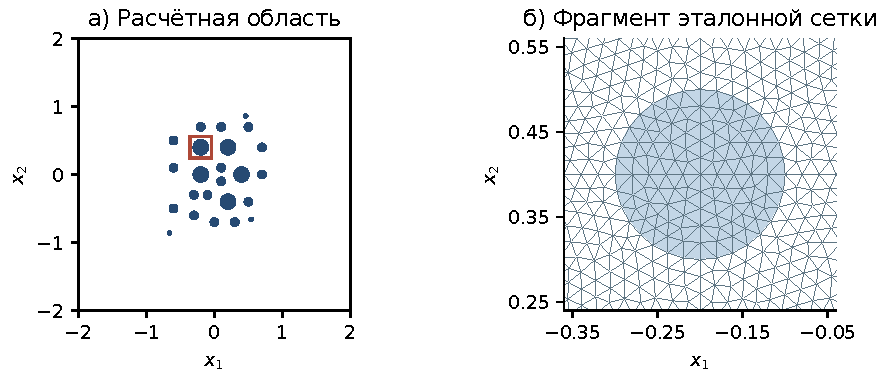
\includegraphics[width=.79\linewidth]{figures/mesh.pdf}
\captionof{figure}{Расположение включений и фрагмент эталонной сетки. Квадрат на левом рисунке ограничивает область, показанную справа.}
\label{fig:mesh}
\end{localfigure}

\clearpage
\section{Метод конечных элементов}
Введём пространство $V_h\subset H^1(\Omega;\C)$ непрерывных кусочно-линейных функций на треугольной сетке. Границы материалов проходят по рёбрам элементов. Обозначим через $u_h$ приближение рассеянного поля $u_s$. Умножим уравнение для $u_s$ на комплексно-сопряжённую тестовую функцию $\overline v_h$, проинтегрируем по частям и учтём условие~\eqref{eq:pde}. Получим вариационную задачу. Требуется найти $u_h\in V_h$, удовлетворяющее для всех $v_h\in V_h$ равенству
\begin{align}
 &\int_\Omega \alpha\nabla u_h\cdot\nabla\overline v_h\,dx
   -k^2\int_\Omega n u_h\overline v_h\,dx
   -\ii k\int_{\partial\Omega}u_h\overline v_h\,ds \nonumber\\
 &\qquad= \int_\Omega(1-\alpha)\nabla u_i\cdot\nabla\overline v_h\,dx
          +k^2\int_\Omega(n-1)u_i\overline v_h\,dx . \label{eq:weak}
\end{align}
Оба слагаемых в правой части обращаются в нуль в фоновом материале. Поэтому при сборке вектора нагрузки можно ограничиться элементами включений, сохраняя вклад скачков коэффициентов в слабой постановке.

Обозначим через $K_\alpha$, $M_n$ и $B$ матрицу жёсткости с весом $\alpha$, матрицу масс с весом $n$ и граничную матрицу масс. Для вектора узловых значений $U_h$ задача~\eqref{eq:weak} принимает вид
\begin{equation}
 A_h(k)U_h=F_h(k,\theta),\qquad A_h(k)=K_\alpha-k^2M_n-\ii kB.
 \label{eq:algebra}
\end{equation}
Эталонная сетка с заданным шагом $h=0{,}02$ содержит 53\,246 узлов и 105\,690 треугольников. Все эталонные поля рассчитаны на этой сетке. Скалярное произведение узловых полей зададим согласованной матрицей масс $M$ с единичным весом. Тогда $\norm{z}_M^2=z^*Mz$ равно квадрату нормы соответствующей кусочно-линейной функции в $L^2(\Omega)$.

\subsection*{Многомасштабное пространство GMsFEM}
Разобьём $\Omega$ на $20\times20$ квадратов. Для построения базиса используется вспомогательная треугольная сетка с шагом $0{,}04$ и 17\,549 неизвестными. В окрестности $\omega_p$ крупной вершины $p$ решим локальные задачи с узловыми граничными данными. На одном граничном узле значение равно единице, на остальных равно нулю. Для базиса типа~1 используется оператор $-\nabla\!\cdot(\alpha\nabla)$, для типа~2 к нему добавляется член $-k^2n$. Полученные решения образуют столбцы $\Psi_p$. В их пространстве рассмотрим задачу
\begin{equation}
  (\Psi_p^*K_{\alpha,p}\Psi_p)z_j
   =\lambda_j(\Psi_p^*M_{\alpha,p}\Psi_p)z_j ,
 \label{eq:local}
\end{equation}
где $K_{\alpha,p}$ и $M_{\alpha,p}$ обозначают локальные матрицы жёсткости и масс с весом $\alpha$. Оставим $m$ собственных векторов, отвечающих наименьшим собственным значениям. Умножим $\Psi_pz_j$ в узлах на вершинную функцию. Её получаем, решая внутри каждого крупного квадрата задачу соответствующего типа со следом билинейной вершинной функции на границе. Соберём полученные функции в матрицу $P$. Вместо полной системы на вспомогательной сетке решается система Галёркина
\[
  (P^* A_{0{,}04}(k)P)y=P^*F_{0{,}04}(k,\theta),\qquad U_{\rm ms}=Py .
\]
Здесь индекс $0{,}04$ указывает на матрицу и правую часть, собранные на вспомогательной сетке. На 441 крупной вершине сохраняется по $m$ локальных функций, поэтому размер системы равен $441m$. Базис типа~1 общий для всех $k$. Базис типа~2 строится для каждого $k$ и используется для всех восьми направлений при этом волновом числе.

\clearpage
\section{Метод сингулярного разложения (SVD)}
Пусть $f^{(s)}\in\R^{N_h}$ обозначает узловой вектор действительной части решения для $s$-го обучающего примера, $N_h=53\,246$. Для мнимой части выполним те же построения независимо. По $N$ обучающим векторам найдём среднее $\bar f$ и составим матрицу $X\in\R^{N\times N_h}$, строки которой равны $(f^{(s)}-\bar f)^\T$. Сингулярные числа матрицы $XM^{1/2}$ и её правые сингулярные векторы определяют разложение в метрике МКЭ. Так как $N\ll N_h$, применим метод снимков~\cite{sirovich}:
\begin{equation}
  XMX^\T v_j=\sigma_j^2 v_j,\qquad
  \phi_j=\sigma_j^{-1}X^\T v_j,\qquad
  \phi_i^\T M\phi_j=\delta_{ij}.
  \label{eq:pod}
\end{equation}
Векторы $v_j$ евклидово ортонормированы, сингулярные числа расположены по убыванию. Обозначим $\Phi_r=(\phi_1,\ldots,\phi_r)$. Для произвольного снимка $f$ его коэффициенты и восстановление определяются формулами
\begin{equation}
 c=\Phi_r^\T M(f-\bar f),\qquad f_r=\bar f+\Phi_r c .
 \label{eq:project}
\end{equation}
Такое восстановление даёт наименьшую погрешность в норме $M$ в выбранном аффинном пространстве. Для комплексного поля получаем два базиса по $r$ мод и $2r$ вещественных коэффициентов. При изменении $N$ средние поля и базисы пересчитываются по соответствующей обучающей выборке.

\section{Метод спектрального нейрооператора (SNO)}
В рассматриваемом варианте спектрального нейрооператора~\cite{fanaskov} по параметрам падающей волны определяются коэффициенты поля в базисах~\eqref{eq:pod}. Вход для каждой моды имеет вид $(0,0,\cos\theta,\sin\theta,\widetilde k)$, где $\widetilde k=(k-\bar k)/s_k$. Среднее $\bar k$ и стандартное отклонение $s_k$ вычисляются по обучающей выборке. Две нулевые компоненты соответствуют фиксированным полям материала.

Общий для всех строк линейный слой с активацией GELU даёт $Z_0\in\R^{r\times w}$, где $w$ есть ширина слоя. Затем последовательно применяются четыре блока с собственными матрицами (рис.~\ref{fig:architecture}). Каждый блок вычисляет
\begin{equation}
 Z' = Z+\operatorname{GELU}\!\left(ZW_1+\mathbf1 b^\T+DZW_2\right).
 \label{eq:block}
\end{equation}
Матрица $D\in\R^{r\times r}$ смешивает моды, а $W_1,W_2\in\R^{w\times w}$ действуют по признакам. Выходной слой даёт по два числа на моду. Умножая их на стандартные отклонения соответствующих коэффициентов в обучающей выборке и применяя~\eqref{eq:project} отдельно к действительной и мнимой частям, получаем комплексное поле $\widehat U$.

Четыре блока и два линейных слоя содержат $P_{\rm net}=4(2w^2+w+r^2)+8w+2$ обучаемых параметров. Средние поля и базисы SVD фиксируются до обучения сети.

\begin{localfigure}
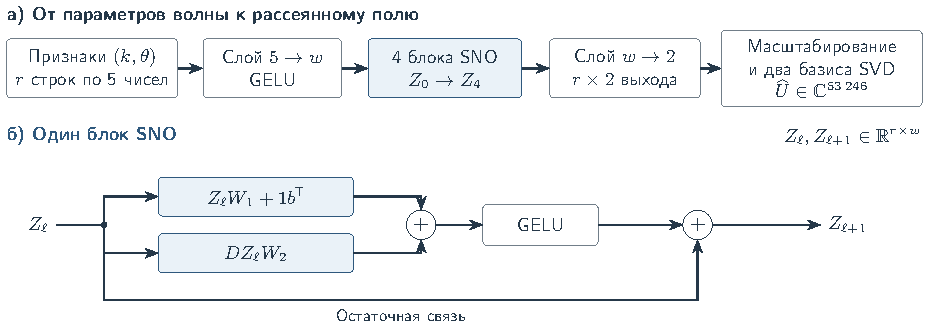
\includegraphics[width=.99\linewidth]{figures/architecture.pdf}
\captionof{figure}{Архитектура SVD-SNO. Внутри блока верхняя ветвь преобразует признаки каждой моды, нижняя смешивает моды. Знак «$+$» обозначает поэлементное сложение.}
\label{fig:architecture}
\end{localfigure}

\clearpage
\section{Вычислительная реализация}
Для каждого $k$ заданы восемь углов $\theta_j=(j+1/2)\pi/4$, $j=0,\ldots,7$. Первые 50 обучающих частот равномерно покрывают $[0{,}1;4]$, включая концы отрезка. Затем в наиболее длинные промежутки между соседними частотами добавляются точки вблизи их середин. Так получены вложенные наборы из 50, 75, 100 и 125 частот. Для выбора эпохи и для тестирования независимо заданы ещё по 16 частот. В каждом из 16 равных подынтервалов выбирается по одной точке для каждой выборки. Все восемь направлений одной частоты входят в одну выборку. Таким образом, тест проверяет интерполяцию по $k$ при известных направлениях падения.

Сетка и нумерация степеней свободы считываются средствами DOLFINx. Интегралы с падающей волной вычисляются квадратурой Гаусса $8\times8$ после преобразования треугольника. Матрица~\eqref{eq:algebra} факторизуется в SciPy один раз при каждом $k$, после чего решаются восемь задач с разными правыми частями. Максимальная относительная невязка $\norm{A_hU_h-F_h}_2/\norm{F_h}_2$ по 1\,256 решениям составила $8{,}09\cdot10^{-13}$. Эта величина характеризует решение дискретной системы.

Погрешность каждого приближения оценивается для комплексного рассеянного поля. Через $U_r$ обозначим проекцию его действительной и мнимой частей по~\eqref{eq:project}. Из ортогональности следует
\begin{align}
 e(\widehat U)&=100\,\norm{\widehat U-U_h}_M/\norm{U_h}_M,\label{eq:error}\\
 \norm{\widehat U-U_h}_M^2
 &=\norm{U_h-U_r}_M^2+
 \sum_{a\in\{\mathrm{Re},\mathrm{Im}\}}\norm{\widehat c_a-c_a}_2^2 .\label{eq:loss}
\end{align}
Тождество~\eqref{eq:loss} позволяет обучать сеть в пространстве коэффициентов путём минимизации среднего по пакету значения относительной погрешности. Для каждого тестового поля равенство проверено непосредственным восстановлением узловых значений. Поля GMsFEM и МКЭ со вспомогательной сетки интерполируются в узлы эталонной сетки. Затем для всех методов применяется одна формула~\eqref{eq:error}.

Обучение в PyTorch проводится с новой инициализацией для каждой конфигурации (фиксированное начальное число 2026). Используется метод Adam, размер пакета 64, число эпох 180. По косинусному закону шаг снижается с $0{,}002$ до $0{,}00015$. Для тестирования загружаются веса эпохи с наименьшей средней погрешностью на 128 валидационных полях. Архитектура и длительность обучения одинаковы в серии по $N$; с ростом $N$ увеличивается число обновлений весов за эпоху.

\section{Численные эксперименты}
\subsection*{Размер обучающей выборки}
В табл.~\ref{tab:samples} зафиксированы $r=24$, $w=48$ и $P_{\rm net}=21\,314$. Каждая строка оценивается на одних и тех же 16 тестовых частотах. В столбце «Проекция» указана средняя погрешность $e(U_r)$, в остальных столбцах погрешностей приведены характеристики $e(\widehat U)$ по 128 полям.

\begin{localtable}
\captionof{table}{Погрешность на тестовой выборке при увеличении числа обучающих полей, \%}\label{tab:samples}
\begin{tabular}{rrrrrr}\toprule
Полей $N$ & Частот & Проекция & Средняя SNO & Медиана SNO & 95-й процентиль\\\midrule
\tabinput{tables/samples}\bottomrule
\end{tabular}
\end{localtable}

\clearpage
\subsection*{Число мод и число обучаемых параметров}
При 24 модах средняя погрешность проекции составляет от 14,11 до 14,33\% для четырёх размеров выборки. В то же время погрешность SNO уменьшается с 33,48 до 20,00\%. Следовательно, в этой серии меняется главным образом точность определения коэффициентов. В табл.~\ref{tab:modes} для каждого ранга сравниваются две ширины сети. Обучающие поля и базисы в каждой паре совпадают.

\begin{localtable}
\captionof{table}{Число мод $r$ для каждой компоненты, ширина $w$, число обучаемых параметров и погрешности при $N=1\,000$. Все погрешности в процентах}\label{tab:modes}
\begin{tabular}{rrr rrrr}\toprule
 & & & \multicolumn{1}{c}{Проекция} & \multicolumn{3}{c}{SNO}\\
\cmidrule(lr){5-7}
$r$ & $w$ & $P_{\rm net}$ & тест, средняя & валид., средняя & тест, средняя & тест, $q_{0{,}95}$\\\midrule
\tabinput{tables/modes}\bottomrule
\end{tabular}
\end{localtable}

При $r=12$ само ограничение пространства даёт 46,57\% средней погрешности. Увеличение ширины с 24 до 48 при этом ранге снижает погрешность сети лишь с 50,78 до 47,56\%. При $r=48$ проекция даёт уже 0,48\%, но сеть ширины 24 восстанавливает поле с погрешностью 21,49\%. Увеличение ширины до 48 при том же базисе снижает её до 12,35\%. Согласно~\eqref{eq:loss}, при таком числе мод основная часть погрешности связана с определением коэффициентов. Даже для этой сети 95-й процентиль равен 33,26\%. Среднее значение поэтому недостаточно для описания точности на отдельных задачах.

\subsection*{Сопоставление с GMsFEM}
В табл.~\ref{tab:gms} для GMsFEM указано число локальных мод $m$ на одну крупную вершину и число комплексных неизвестных $N_H$ в системе Галёркина. Отдельно приведён результат полного МКЭ на вспомогательной сетке. Он показывает расхождение с эталоном до многомасштабной редукции. Для сопоставления приведена также сеть с наименьшей валидационной погрешностью из табл.~\ref{tab:modes}.

\begin{localtable}
\captionof{table}{Погрешности относительно эталонного МКЭ на общих 128 тестовых полях, \%. Для SNO $r=48$, $w=48$ и $N=1\,000$}\label{tab:gms}
\begin{tabular}{lrrrrr}\toprule
Метод & $m$ & $N_H$ или $N_h$ & Средняя & Медиана & 95-й процентиль\\\midrule
\tabinput{tables/gms}\midrule
\tabinput{tables/paired_sno}\bottomrule
\end{tabular}
\end{localtable}
При $m=16$ тип~2 даёт среднюю погрешность 7,08\%, тип~1 даёт 21,75\%. Различие сохраняется и при сравнении отдельных решений. Тип~2 с 16 модами оказался точнее сети с $r=w=48$ на 120 из 128 задач. У этого варианта GMsFEM медиана составляет 1,73\%, а 95-й процентиль достигает 31,61\%. У сети с 24 модами наибольшая погрешность в среднем по направлениям составила 48,19\% при $k\approx0{,}325$, у GMsFEM типа~2 с $m=16$ она достигла 45,97\% при $k\approx3{,}687$ (рис.~\ref{fig:errors}).

\clearpage\enlargethispage{.8\baselineskip}
\begin{localfigure}
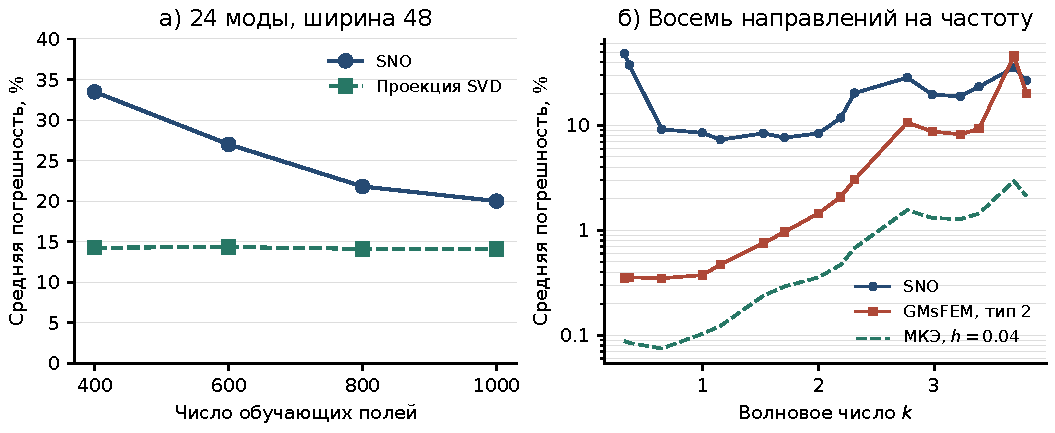
\includegraphics[width=.88\linewidth]{figures/errors.pdf}
\captionof{figure}{Средняя погрешность по 128 полям (а) и по восьми направлениям при каждом $k$ (б). Справа шкала ординат логарифмическая. На панели (б) для SNO взяты $N=1\,000$, $r=24$, $w=48$, для GMsFEM взяты $m=16$ локальных мод.}
\label{fig:errors}
\end{localfigure}
\begin{localfigure}
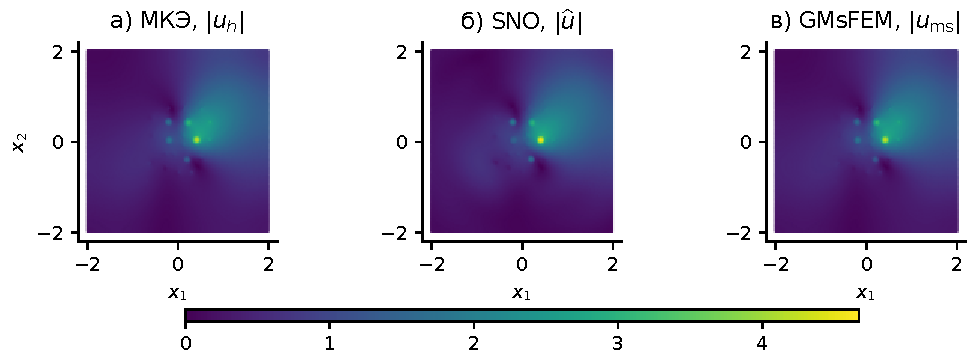
\includegraphics[width=.85\linewidth]{figures/field.pdf}
\captionof{figure}{Модуль рассеянного поля на эталонной сетке при $k=2{,}19157$, $\theta=\pi/8$. Приведены МКЭ, SNO ($N=1\,000$, $r=24$, $w=48$) и GMsFEM (тип~2, $m=16$). Шкала амплитуды общая.}
\label{fig:field}
\end{localfigure}
Для первого направления девятой тестовой частоты (рис.~\ref{fig:field}) погрешность комплексного поля составляет 12,29\% у SNO и 2,17\% у GMsFEM.
\section{Заключение}
При фиксированных ширине сети и числе эпох увеличение числа обучающих полей с 400 до 1\,000 уменьшило среднюю погрешность при 24 модах с 33,48 до 20,00\%. Дальнейшее увеличение числа мод до 48 при $N=1\,000$ уменьшило погрешность проекции до 0,48\%, а погрешность прогноза до 12,35\%. При 48 модах основную часть погрешности даёт приближение коэффициентов.
Вариант GMsFEM с продолжением Гельмгольца и 7\,056 неизвестными дал 7,08\% средней погрешности. Соответствующее значение для полного МКЭ на той же вспомогательной сетке составило 0,82\%. Эти оценки относятся к одной геометрии, одному набору коэффициентов материала и восьми заданным направлениям. Для SNO использована одна инициализация на конфигурацию. Точность относительно решения во внешней неограниченной области требует отдельного исследования.

\begingroup\small\begin{thebibliography}{9}\setlength{\itemsep}{0pt}
\bibitem{kalachikova} Kalachikova U., Vasilyeva M., Harris I., Chung E. T. Generalized Multiscale Finite Element Method for scattering problem in heterogeneous media. \emph{Journal of Computational and Applied Mathematics}. 2023. Vol.~424. 114977. \href{https://doi.org/10.1016/j.cam.2022.114977}{doi:10.1016/j.cam.2022.114977}.
\bibitem{sirovich} Sirovich L. Turbulence and the dynamics of coherent structures. Part I. Coherent structures. \emph{Quarterly of Applied Mathematics}. 1987. Vol.~45. P.~561--571. \href{https://doi.org/10.1090/qam/910462}{doi:10.1090/qam/910462}.
\bibitem{fanaskov} Fanaskov V., Oseledets I. Spectral Neural Operators. 2022, revised 2024. \href{https://arxiv.org/abs/2205.10573}{arXiv:2205.10573}.
\end{thebibliography}\endgroup
\end{document}
